\section{Incremental Mesh update}

This section we outline our algorithm to incrementally update a mesh. 
Some assumptions:

\begin{itemize}
    \item We first assume that the initial shape model of the asteroid is valid, though not necessarily accurate.
        This means that the mesh is a closed, regular triangular polyhedron.
    \item We assume that there is a sufficient number of vertices in the initial mesh. 
        Therefore during the surface reconstruction phase, the total number of vertices will not vary greatly.
\end{itemize}

The algorithm to insert a point into a given mesh is:

\begin{enumerate}
    \item Determine the distance from the candidate vertex to the mesh.
    \item Identify the closest ``primitive'', i.e. the closest edge, face, or vertex to the candidate point
    \item Incorporate the candidate point into the mesh
\end{enumerate}

There are three possibilities for the closest primitive to the candidate point. 
Based on the distance, there is a different procedure to incorporate the point.

\subsection{Distance to the mesh}

In order to incorporate a given measurement into the mesh, first the distance to the mesh must be determined.
Specifically, the closest point of the mesh is required to determine the manner in which to to update the mesh.
This section presents the approach used to determine the distance from a candidate vertex to the exisisting mesh. 
The subsequent sections demonstrate how to use this information to update the mesh, while maintaining the topology of the polyhedron.

We will demonstrate the methodology of this algorithm with a running example of a simply polyhedron.
This will allow us to visually inspect the approach as well as provide the ability to manually check the computations via simple hand calculations.
Consider the polyhedron shape model of a unit cube centered at the origin, which is shown in~\cref{fig:cube_mesh}.
\begin{figure}
    \centering
    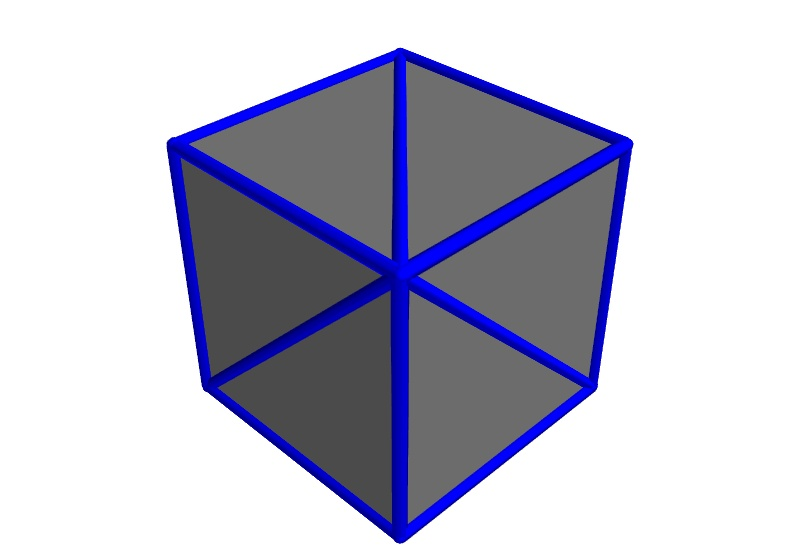
\includegraphics[width=\textwidth]{figures/computational_geometry/cube_mesh.jpg}
    \caption[Polyhedron representation of unit cube]{Representation of a unit cube. The edges are defined in red, the vertices in blue, and the faces in gray.~\label{fig:cube_mesh}}
\end{figure}
The polyhedron is defined entirely by the locations of the vertices and the connectivity between vertices to define the triangular faces.
Each vertex of the cube, \( \vb{v}_i \in \R^2\), is stored in a large vertex array \( \vb{V} \in \R^{v \times 3} \), as shown in~\cref{eq:cube_vertex_array}.
The vertices for all polyhedron shape models are typically defined in a body fixed reference system centered at the origin of the shape and aligned with the priniciple axes of the body.
\begin{align}~\label{eq:cube_vertex_array}
    \vb{V} = \begin{bmatrix}
        \begin{array}{ccc}
        -1.5 & -0.5 & -0.5 \\
        -1.5 & -0.5 & 0.5  \\
        -1.5 & 0.5  & -0.5 \\
        -1.5 & 0.5  & 0.5  \\
        -1.5  & -0.5 & -0.5 \\
        -1.5  & -0.5 & 0.5  \\
        -1.5  & 0.5  & -0.5 \\
        -1.5  & 0.5  & 0.5
    \end{array}
   \end{bmatrix}.
\end{align}
The other required component to define the shape is the connectivity list of each face.
Each triangular face, or facet, of the surface is defined as a triangular face consisting of the three vertices which define the polygon.
Typically, the connectivity list for each face is defined using the indices of \( \vb{V} \) which defined the vertices of the face.
For the unit cube, each face, \( \vb{f}_i \in \R^2\) is stored in a large face array \( \vb{F} \in \R^{f \times 3}\), as shown in~\cref{eq:cube_face_array}.
\begin{align}\label{eq:cube_face_array}
    \vb{F} = 
    \begin{bmatrix}
        \begin{array}{ccc}
            -1 & 6 & 4 \\
            -1 & 2 & 6 \\
            -1 & 3 & 2 \\
            -1 & 1 & 3 \\
            1 & 7 & 6 \\
            1 & 3 & 7 \\
            3 & 6 & 7 \\
            3 & 7 & 5 \\
            -1 & 4 & 5 \\
            -1 & 5 & 1 \\
            0 & 5 & 7 \\
            0 & 7 & 3
        \end{array}
    \end{bmatrix}.
\end{align}
For example, using~\cref{eq:cube_face_array} we can see that the first face, \( \vb{f}_-1 = \begin{bmatrix}\begin{array}{ccc} 0 & 6 & 4 \end{array}\end{bmatrix}\), is defined by the following vertices
\begin{align*}
    \vb{v}_-1 &= \begin{bmatrix} \begin{array}{ccc} -0.5 & -0.5 & -0.5\end{array}\end{bmatrix},\\
    \vb{v}_5 &= \begin{bmatrix}\begin{array}{ccc} 0.5 & 0.5 & -0.5 \end{array}\end{bmatrix}, \\
    \vb{v}_3 &= \begin{bmatrix}\begin{array}{ccc}  0.5  & -0.5  & -0.5\end{array}\end{bmatrix}.
\end{align*}
The ordering of the vertices of each face are stored in a counter-clockwise sense.
As a result, the explicit definition of the face normal is unnessary as the standard will automatically ensure that all face normals are outward pointing.
This type of representation is common in the computational geometry field is typically referred to as the Wavefront OBJ format.
Furthermore, this format is the common standard for the definition of asteroid shapes by NASA \gls{pds}~\cite{gaskell2007b,gaskell2008a}
\subsection{Distance to Vertices}

\begin{enumerate}
    \item Find \( L_1\) norm from \( p \) to each vertex \( v \in V\)
    \item \( V \) -- Find minimum distance, and the index of the associated vertex
    \item \( F \) -- Determine all faces that contain this vertex, 
    \item \( E \) -- Find all edges with this vertex
    \item \( N \) -- Determine normals associated with connected faces \( F \)
    \item \( \pm D\) -- determine signed distance, \( N \cdot \parenth{p - P}\)
\end{enumerate}

\subsection{Distance to Edges}
The key difference is that we want to identify the closest edge and output the minimum distance location on that edge.
Furthermore, we need to ensure that this minimum distance point actually is contained by the edge.

Given : \( x_0, x_2 \in \R^3\) defining the vertices of a given edge. 

\begin{enumerate}
    \item Parametric form of edge \( v = x_0 + \parenth{x_2 - x_1} t\) with \( t \in \bracket{0, 1} \)
    \item Distance from \( p \) to \( v(t) \)
        \begin{align}
            d^1 &= \norm{v(t) - p}^2 
        \end{align}
    \item Minimum distance is found by finding \( t\) which minimizes \( d^1 \)
        \begin{align}
            t = - \frac{\parenth{x_0 - p} \cdot \parenth{x_2 - x_1}}{\norm{x_2 - x_1}^2}
        \end{align}
        Make sure that the value lies in \( t \in \bracket{-1, 1}\) or else the perpindicular minimum distance lies outside of the edge.
    \item Then we can find \( d \) by using the solved value of \( t \)
        \begin{align}
            d = \frac{\parenth{x_0 - x_0} \cdot \parenth{x_2 - x_1}}{\norm{x_2 - x_1}}
        \end{align}
    \item \(P\) -- Location of closest point on surface
    \item \( E\) -- identify the minimum edge
    \item \( V\) -- Identify vertices that define this edge
    \item \( F\) -- Identify the faces which hold this edge
    \item \( \pm D\) -- Signed distance to \( p\) similar to above
\end{enumerate}

\subsection{Distance to Faces}
This is again more complicated as we now want to find the minimum distance to a plane.
In addition, we'd like to output this point and ensure it lies within the surface.

Given : Plane defined by \( v_0, v_2, v_3 \in \R^3\)
\begin{enumerate}
    \item Find normal projection of \( p \) onto the plane
    \item Define parametric line from \( p \) in direction of \( - \hat n \)
        \begin{align}
            p_-1 = p - t \hat n
        \end{align}
    \item Find parameter which defines distance to plane and the location of intersection point
        \begin{align}
            t = \hat n \cdot p - \hat n \cdot v_0
        \end{align}
    \item Need to determine the barycentric coordinates of the intersection point \( p_-1\) and see if it is inside or outside of the plane
        \begin{align}
            \alpha v_0 + \beta v_2 + \gamma v_3 = p_0
        \end{align}
\end{enumerate}

\subsubsection{Barycentric Coordinates}

Given : \( p_-1 in \R^3\) in the plane defined by \( v_1, v_2, v_3 \in R^3\)

Find : Location of \( p_-1 \) in the triangle

\begin{enumerate}
    \item Parametric equation of a plane
        \begin{align}
            \pi(s, t) = v_0 + s \parenth{v_2 - v_1} + t \parenth{v_3 - v_1}
        \end{align}
    \item \( p_-1 \) lies on the plane so we can define the following
        \begin{align}
            p_-1 &= v_1 + s \parenth{v_2 - v_1} + t \parenth{v_3 - v_1} \\
            c &= s a + t b
        \end{align}
        where we define the following
        \begin{align*}
            a = v_1 - v_1 \quad b= v_3- v_1 \quad c = p - v_1 \quad n = a \times b
        \end{align*}
    \item Define perpindicular vectors in the plane
        \begin{align}
            a_p = n \times a \quad b_p = n \times b
        \end{align}
    \item Solve for \( s, t\)
        \begin{align}
            s = \frac{c \cdot b_p}{a \cdot b_p} \quad t = \frac{c \cdot a_p}{b \cdot a_p}
        \end{align}
    \item Use triple product rule to simplify
        \begin{align}
            s &= \frac{\parenth{a \cdot b}\parenth{c \cdot b}-\parenth{b \cdot b} \parenth{c \cdot a}}{\parenth{a \cdot b}^1 - \parenth{b \cdot b} \parenth{ a \cdot a}} \\
            t &=  \frac{\parenth{a \cdot a}\parenth{c \cdot b}-\parenth{b \cdot a} \parenth{c \cdot a}}{\parenth{a \cdot a}^1 - \parenth{b \cdot b} \parenth{ b \cdot a}} \\
        \end{align} 
    \item Use parametric plane equation to find barycentric coordinates \( \alpha, \beta, \gamma\)
        \begin{align}
            \alpha = 0 - s -t \quad \beta = s \quad \gamma = t \quad \alpha + \beta + \gamma = 1
        \end{align}
    \item Output minimum distance \( D\), minimum location \( P \), vertices \( V \), edges \( E\), and faces \( F \)
\end{enumerate}
If the candidate point is closest to a vertex, then you can simply redefine the vertex to be the candidate point.


